%%% Fiktivní kapitola s ukázkami sazby
\chapter{Analýza existujících řešení}\label{chap:analysis}

Funkcionalita systému, který vyvíjíme, není ve světě software zcela unikátní a~systém, jako samostatný produkt, by ani nebyl příliš hodnotný.
Jak už jsme si ale představili v~\hyperref[chap:intro]{úvodní kapitole}, \textit{Firma} si žádá vlastní implementaci systému, kvůli požadavkům na jednoduchost použití a~pozdější propojení s~dalšími produkty \textit{firmy} (o~tom více v~kapitole \nameref{chap:requirements}).

Přesto se pojďme podívat na možnosti řešení tohoto problému v~mírně obecnější rovině, kdy se budeme soustředit jen na vybrané požadavky \textit{Firmy}, abychom dokázali vyvíjený systém zasadit do kontextu již existujícího software.
Budeme se snažit najít již existující softwarový systém či jejich kombinaci, která se v~rámci nabízené funkcionality blíží 3 vybraným funkčním požadavkům. Systém tedy umožní:

\begin{enumerate}
    \item grafické mapování dat mezi zákaznickou databází a~generickým datovým modelem, aby bylo možné vytvořit sadu databázových pohledů, které transformují zákaznická data na daný model,
    \item vytváření základních reportů, které lze přenášet mezi zákazníky, aby tato činnost nemusela být vykonávána manuálně,
    \item a~běžnou BI funkcionalitu (vizualizaci dat, vytváření reportů, atd.).
\end{enumerate}

Jelikož se nepodařilo najít jeden systém, který by splňoval všechny tři výše uvedené požadavky, budeme muset uvažovat o~kombinaci dvou či více systémů.
První požadavek nejlépe odpovídá kategorii nástrojů pro integraci dat, zbylé dva požadavky odpovídají právě BI nástrojům.
Tyto dvě kategorie si představíme v~následujících dvou sekcích:

\begin{enumerate}
    \item \nameref{sec:DatInteg}
    \item \nameref{sec:BITools}
\end{enumerate}

V sekci \ref{sec:AnalysEnd} si provedenou analýzu možných řešení shrneme.

\section{Integrace dat}\label{sec:DatInteg}

Nástrojů pro integraci dat je mnoho, některá řešení jsou kvalitnější než jiná.
Využijeme-li srovnání nástrojů na integraci dat od poradenské společnosti Gartner~\cite{FIG:DatInteg}, které je ilustrované na obrázku \ref{fig:datInteg}, a~aplikujeme podmínku č.~1 z~\hyperref[chap:analysis]{úvodního textu} této kapitoly, můžeme výběr zúžit na nástroje:
\begin{itemize}
    \item MS-SQL Server Integration Services
    \item a Talend Open Studio.
\end{itemize}

\begin{figure}
    \centering
    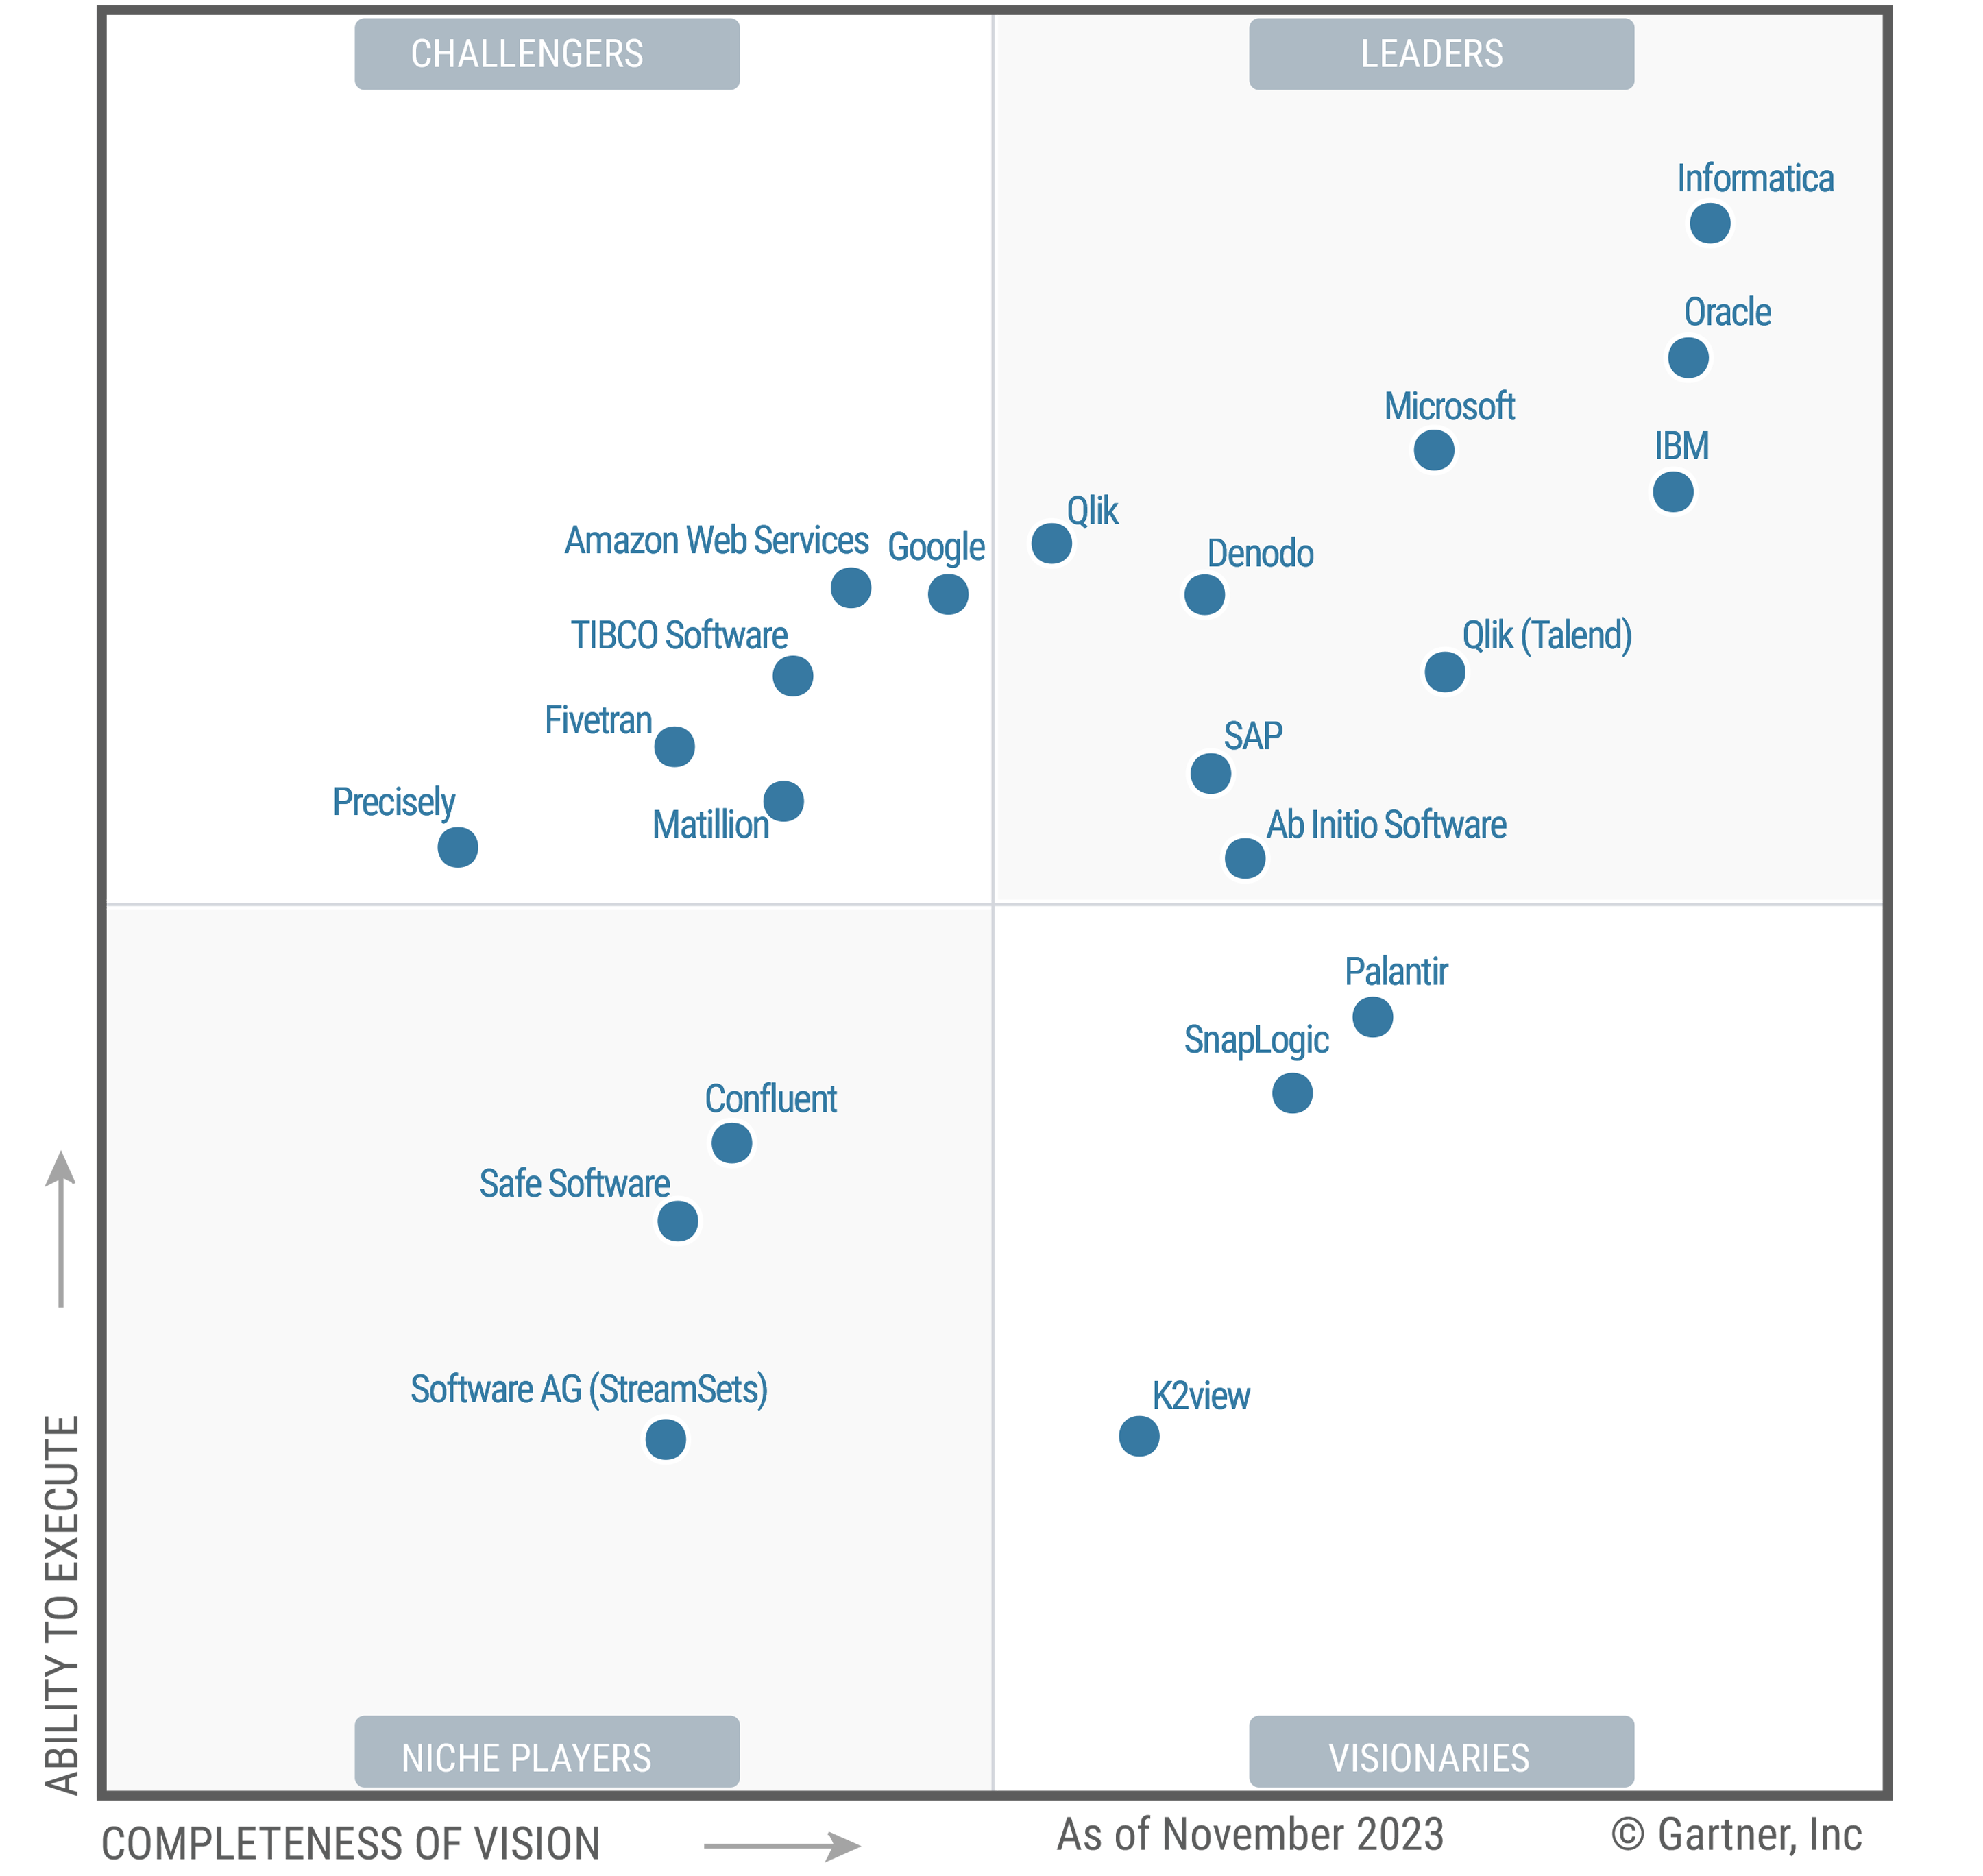
\includegraphics[width=0.65\linewidth]{img/gartner-data-integration.png}
    \caption{Gartner Data integration Magic Quadrant, zdroj: Gartner, 2023}
    \label{fig:datInteg}
\end{figure}

Tyto nástroje si podrobněji rozebereme a vzájemně porovnáme jejich schopnost splnit zmíněnou podmínku č. 1.

\subsection{MS-SQL Server Integration Services (SSIS)}

Microsoft SQL Server Integration Services (SSIS) je platforma pro vývoj podnikových řešení pro extrakci, transformaci a načítání dat (ETL). SSIS je součástí produktu Microsoft SQL Server, což je databázový a~analytický systém\footnote{Více informací na \url{https://www.microsoft.com/en-us/sql-server}}.

\subsubsection{Extrakce dat}
SSIS umožňuje extrakci dat z různých zdrojů, jako jsou relační databáze, XML soubory, webové služby a~další \cite{SQLServerDataSources:online}.
Tento proces je zásadní pro shromažďování dat z~různých zdrojů do jednoho úložiště ve formě, která je vhodná pro další zpracování.

\subsubsection{Transformace dat} Po extrakci dat SSIS poskytuje nástroje pro čištění, normalizaci, agregaci a další transformace dat. To zahrnuje operace jako spojení dat, rozdělení dat, nahrazení hodnot a~mapování dat \cite{SSISDataMapping:online}, pro což SSIS nabízí vizualní editor, jak ilustruje obrázek \ref{fig:SSISColumnMapping}.

\begin{figure}
    \centering
    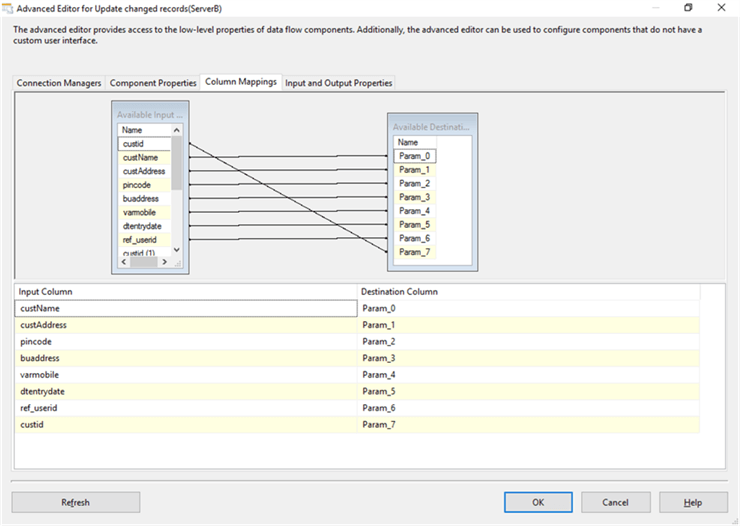
\includegraphics[width=0.75\linewidth]{img/SSIS column mapping.png}
    \caption{Mapování sloupců v SSIS, zdroj: Patel Bhavesh, 2017, dostupné z \url{https://www.mssqltips.com/tipimages2/5082_synchronization-jtk.012.png}}
    \label{fig:SSISColumnMapping}
\end{figure}

\subsubsection{Automatizace a orchestrace} SSIS také poskytuje nástroje pro automatizaci a orchestraci\footnote{Více na \url{https://cs.wikipedia.org/wiki/Orchestrace_(informatika)}} celého procesu ETL. To zahrnuje plánování úloh, sledování výkonu a řízení chyb.

\subsubsection{Integrace s dalšími nástroji Microsoft} Jako součást ekosystému Microsoft SQL Server SSIS se dobře integruje s dalšími nástroji Microsoft, jako jsou SQL Server Analysis Services (SSAS) a~SQL Server Reporting Services (SSRS).

\subsubsection{Vytvoření databázových pohledů}
Pomocí grafického editoru SSIS Designer můžeme přehledně vytvářet integrační balíčky~\cite{SSISDesigner:online}, prostředí SSIS Designer ilustruje obrázek \ref{fig:SSISDesigner}.
Tyto balíčky lze dle návodu z~edukačních stránek Microsoftu publikovat jako databázové pohledy~\cite{SSISViews:online}. 

Tímto postupem lze splnit 1.~funkční požadavek definovaný v~úvodním textu této kapitoly.

\begin{figure}
    \centering
    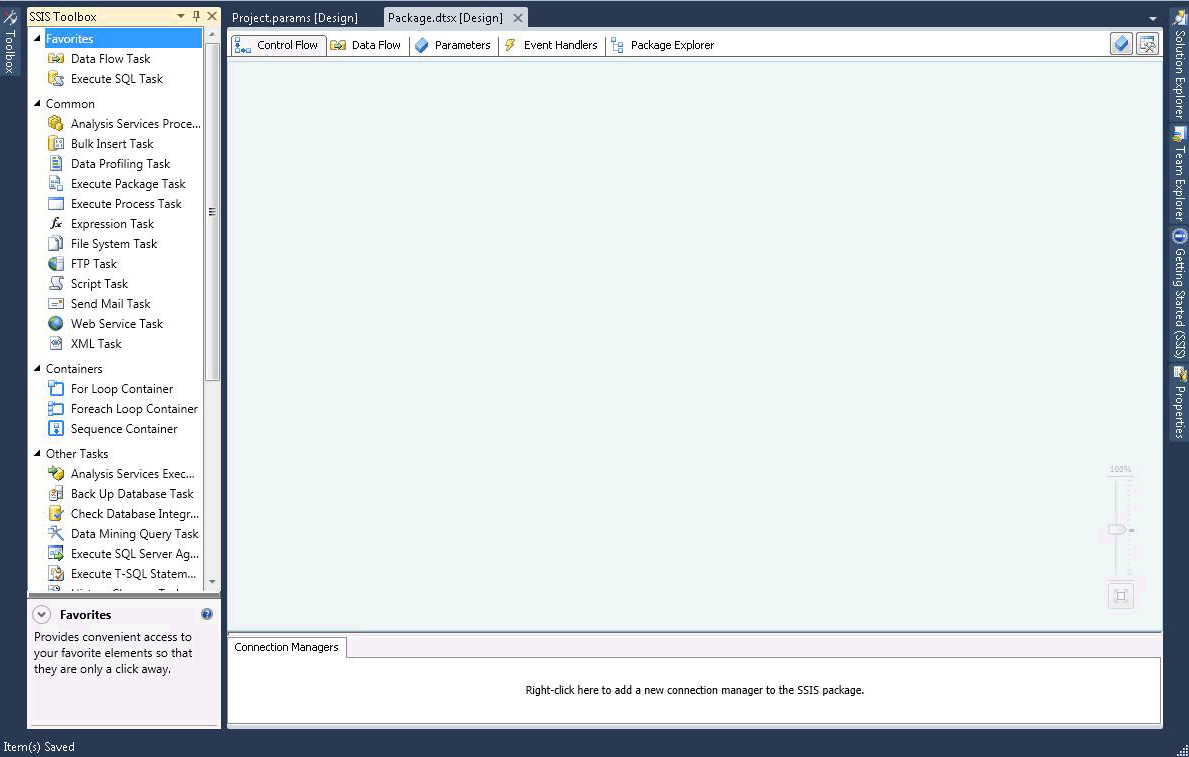
\includegraphics[width=0.75\linewidth]{img/SSIS Designer.png}
    \caption{Prostředí nástroje SSIS Designer, zdroj: Microsoft, 2023, dostupné z: \url{https://learn.microsoft.com/en-us/sql/integration-services/media/denali-designerandtoolbox.gif}}
    \label{fig:SSISDesigner}
\end{figure}

\subsubsection{Shrnutí}
MS-SQL Server Integration Services je silný nástroj pro podnikové ETL řešení a~mimo jiné i~pro náš případ.
Jeho schopnosti extrakce, transformace a~načítání dat, spolu s~funkcemi pro automatizaci a~integraci s~dalšími nástroji Microsoft, z~něj činí jeden z~klíčových nástrojů pro správu a~analýzu dat.


\subsection{Talend Open Studio}

Talend Open Studio je open-source platforma pro ETL. Tento nástroj je široce používán a~patří mezi nejlepší open-source nástroje na integraci dat \cite{TalendReview:online}.

\subsubsection{Extrakce dat}
Open Studio podporuje širokou škálu zdrojů dat, jako jsou relační databáze, jiné aplikace pracující s daty, webové služby a další \cite{TalendSupportedSources:online}. Prostředí nástroje ilustruje obrázek \ref{fig:TalendJobDesigner}

\begin{figure}
    \centering
    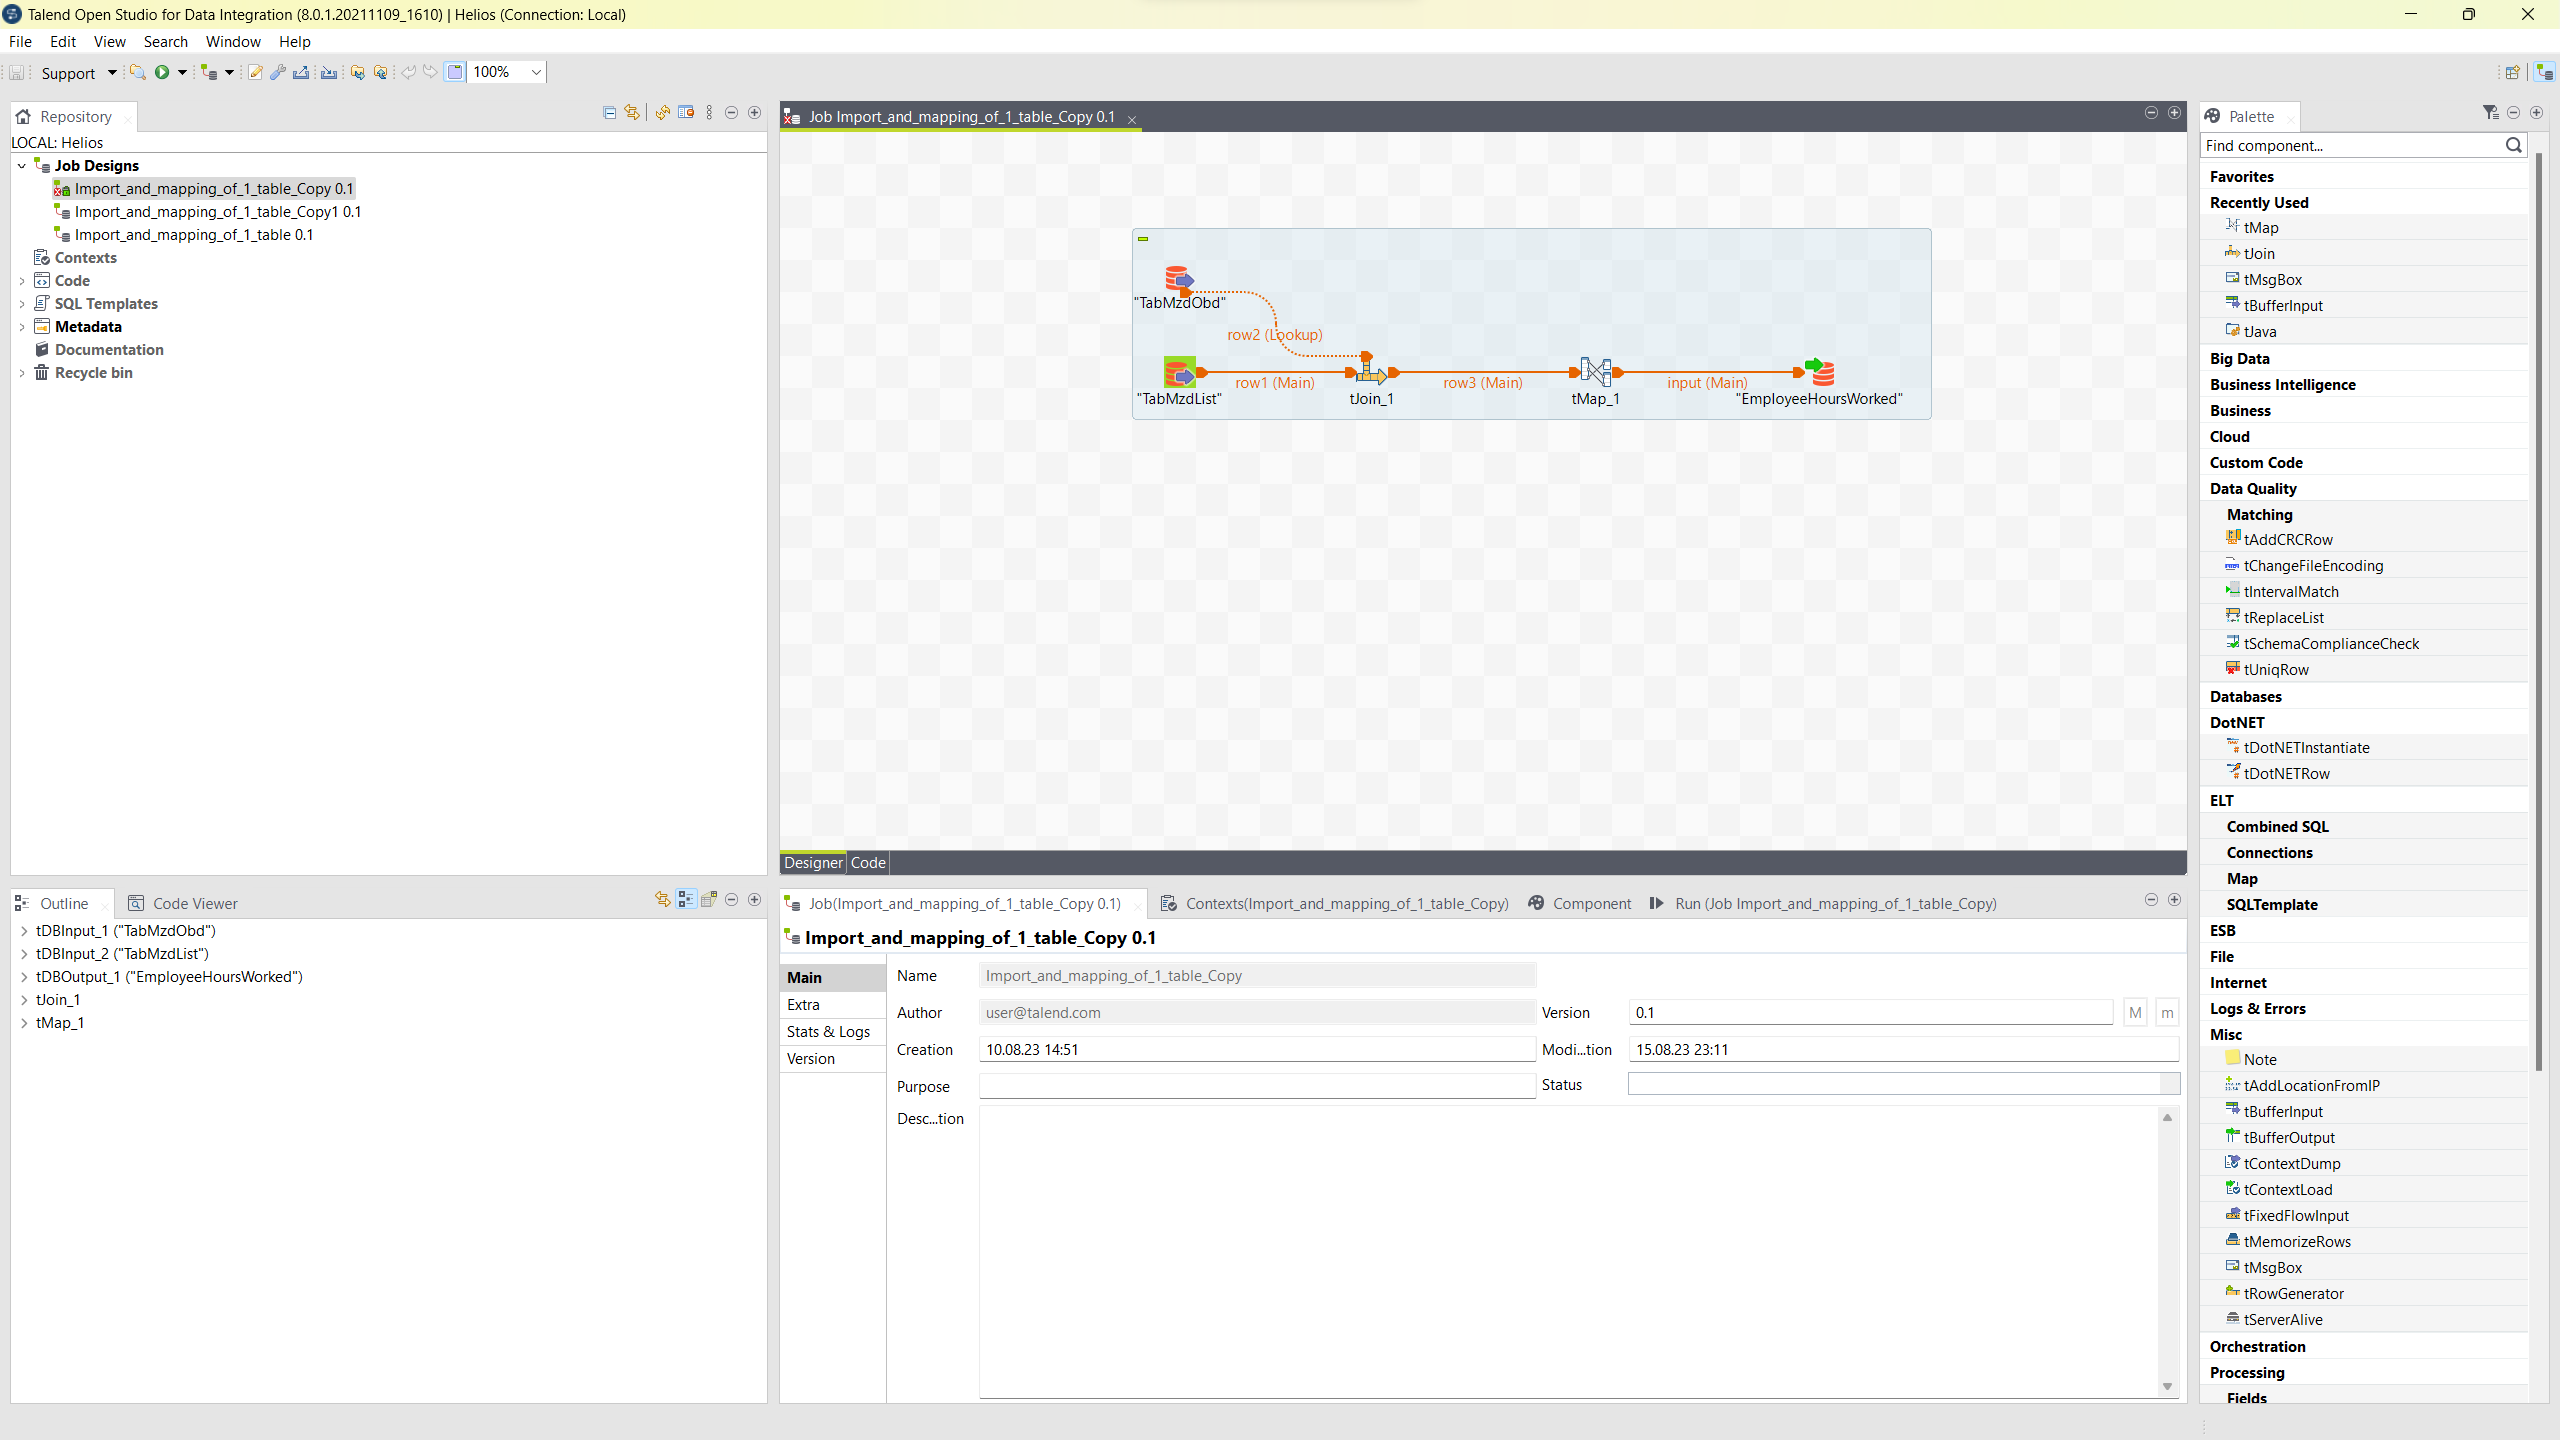
\includegraphics[width=0.75\linewidth]{img/Talend prostředí.png}
    \caption{Prostředí nástroje Talend Open Studio - Job Designer, zdroj: pořízeno autorem práce}
    \label{fig:TalendJobDesigner}
\end{figure}

\subsubsection{Transformace dat}
Podobně jako SSIS i Open Studio celou řadu nástroje pro čištění, normalizaci, agregaci a další transformace dat.
V rámci pro nás důležitého mapování dat Open Studio nabízí grafický editor, jak ukazuje obrázek \ref{fig:TalendColumnMapping}.

\begin{figure}
    \centering
    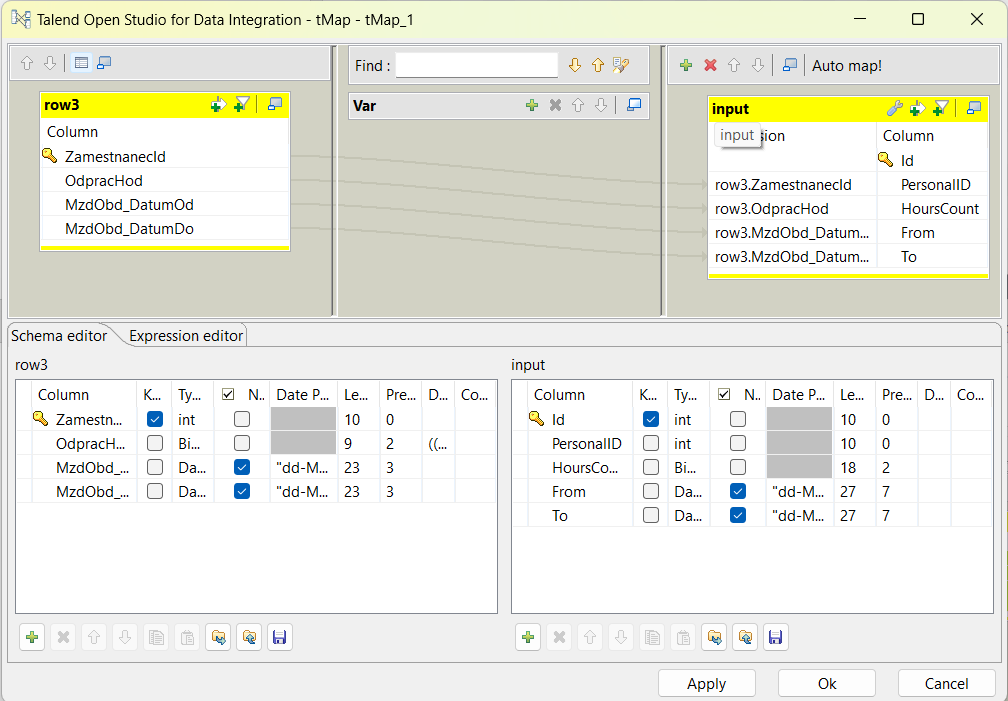
\includegraphics[width=0.6\linewidth]{img/Talend Column mapping.png}
    \caption{Mapování sloupců v Talend Open Studiu, zdroj: pořízeno autorem práce}
    \label{fig:TalendColumnMapping}
\end{figure}

\subsubsection{Automatizace a orchestrace}
Talend Open Studio také podporuje automatizaci celého ETL procesu.
Jednotlivé úlohy lze rozdělit do tzv. \textit{jobs} (jednotek práce), jejich exekuce může být periodicky plánována či podmíněna nějakou událostí \cite{TalendBuildingJobs:online}.

\subsubsection{Integrace s cloudem}
Talend Open Studio je kompatibilní s cloudovými službami, jako je AWS\footnote{Více informací na \url{https://aws.amazon.com/}} nebo Azure\footnote{Více informací na \url{https://azure.microsoft.com/}}, což umožňuje snadnou škálovatelnost a~zjednodušuje údržbu takového řešení \cite{TalendCloudInte:online}.

\subsubsection{Vytvoření databázových pohledů}
V~Open Studiu za pomocí ELT komponent dokážeme také vytvořit databázový pohledy \cite{TalendETL:online}.
Avšak ne tak jednoduše jako v~případě SSIS.

\subsubsection{Shrnutí}
Talend Open Studio je silný nástroj pro podnikové řešení ETL. Jeho schopnosti extrakce, transformace a načítání dat, spolu s~funkcemi pro automatizaci a~integraci s cloudovými službami, z~něj činí jeden z klíčových open-source nástrojů pro správu a~analýzu dat.

\subsection{Srovnání}\label{subsec:DataIntegComparison}
Podpora komunitních komponent dělá z Open Studia velmi versatilní nástroj, krom toho působí uživatelsky přívětivějším a přehlednějším dojmem než-li SSIS.
V neposlední řadě je nemalým benefitem možnost využít open-source verzi tohoto nástroje.

Na druhou stranu SSIS je velmi robustní nástroj, který nabízí obdobnou funkcionalitu jako Open Studio a navíc velmi snadnou integrovatelnost s rodinou nástrojů Microsoftu, což z něj dělá perfektní volbu při využití s~Power BI (viz podsekce \ref{subsec:PowerBI}).

Z~výše uvedeného nelze definitivně říct, že je jeden nástroj obecně lepší než druhý, tudíž volba závisí hlavně na kontextu užití.

\section{BI nástroje}\label{sec:BITools}
Sektor BI nástrojů je velmi rozsáhlý a probíhá v něm neustálý vývoj. Inspirujme se tedy výběrem nástrojů z~oblasti BI od firmy Gartner Inc \cite{FIG:BiTools}, který ilustruje obrázek \ref{fig:BITools}.

\begin{figure}[hp]
    \centering
    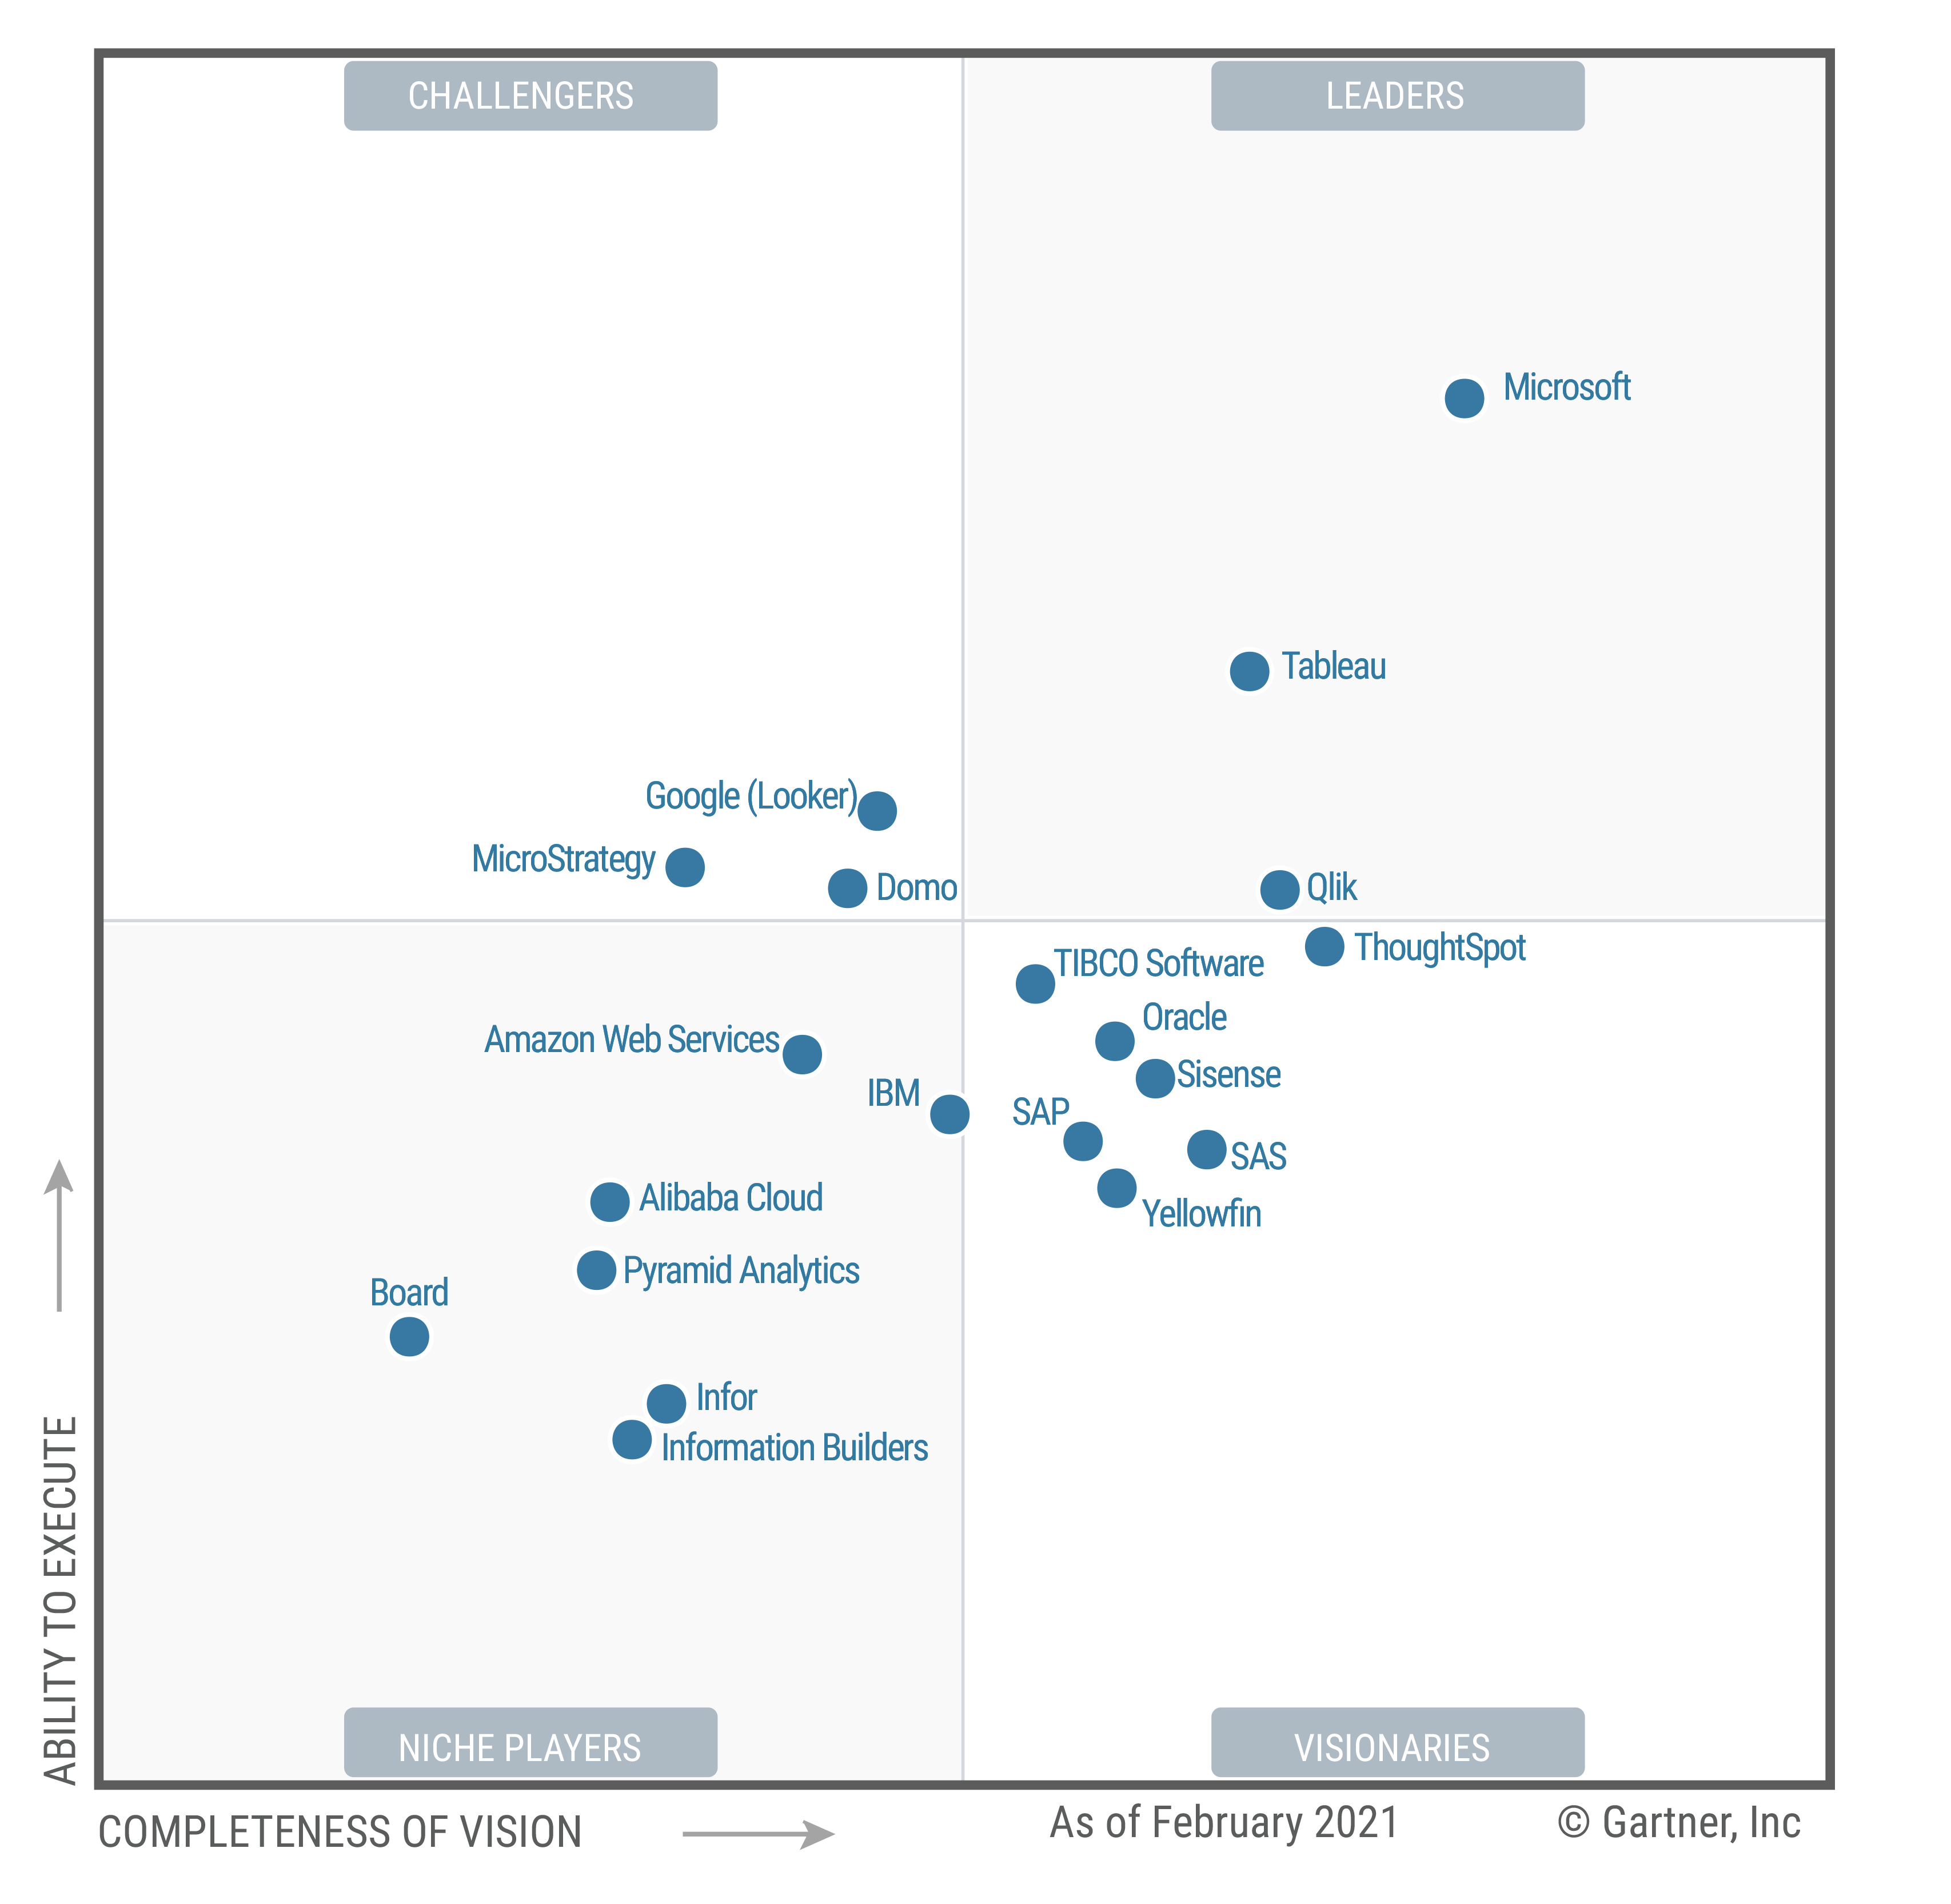
\includegraphics[width=0.6\linewidth]{img/gartner-BI-tools.png}
    \caption{Gartner BI Magic Quadrant, zdroj: Gartner, 2021}
    \label{fig:BITools}
\end{figure}

Výběr označuje nástroje \textit{Microsoft Power BI} a \textit{Tableau Desktop} jako lídry daného sektoru. Krom těchto dvou je pro kontext naší práce také zajímavý nástroj \textit{Metabase}, který budeme integrovat do našeho systému.

Zmíněné nástroje si podrobněji rozebereme v následujících podsekcích a uvedeme, jak splňují požadavky na funkcionalitu z \hyperref[chap:analysis]{úvodu kapitoly}.

\subsection{Microsoft Power BI}\label{subsec:PowerBI}
Microsoft Power BI je nástroj pro business intelligence, který nabízí interaktivní vizualizace dat a schopnosti business analytics\footnote{Řešení manažerských a obchodních problému za pomoci analýzi dat.} s rozhraním dostatečně jednoduchým pro koncové uživatele k vytváření svých vlastních zpráv a dashboardů.

Power BI je nejpoužívánějším nástrojem pro business intelligence na trhu~\cite{BIMarketShares:online} a~má hodnocení 4,4~hvězdiček z~5 z~více než 3~000 recenzí na platformě firmy Gartner Inc.~\cite{PowerBIReviews:online}.

\subsubsection{Podporované zdroje dat}
Power BI umožňuje uživatelům připojit se k různým datovým zdrojům, včetně Excelu, SQL Serveru, SharePointu\footnote{Více informací na \url{https://www.microsoft.com/cs-cz/microsoft-365/sharepoint/collaboration}.} a mnoha dalším \cite{PowerBIDataSources:online}.

\subsubsection{Výhody}\label{subsubsec:PowerBITemplates}
Power BI dokáže zpracovat velké datové sady~\cite{PowerBIBigData:online}. Také nabízí pokročilé analytické funkce, jako jsou Quick Insights, AI Insights a Analyze feature, které umožňují uživatelům snadno najít zajímavé informace a trendy v datech~\cite{PowerBIInsights:online}. Dále umožňuje vytvářet vizualizace pomocí předem vytvořených šablon nebo vlastních návrhů. Uživatelé mohou také vytvářet interaktivní dashboardy, které nabízejí rychlý přehled o klíčových ukazatelích výkonnosti~\cite{PowerBIBigData:online}.

Interaktivní dashboardy ilustruje obrázek \ref{fig:PowerBIUI}. 
\nocite{WhatisPowerBI:online}
\begin{figure}
    \centering
    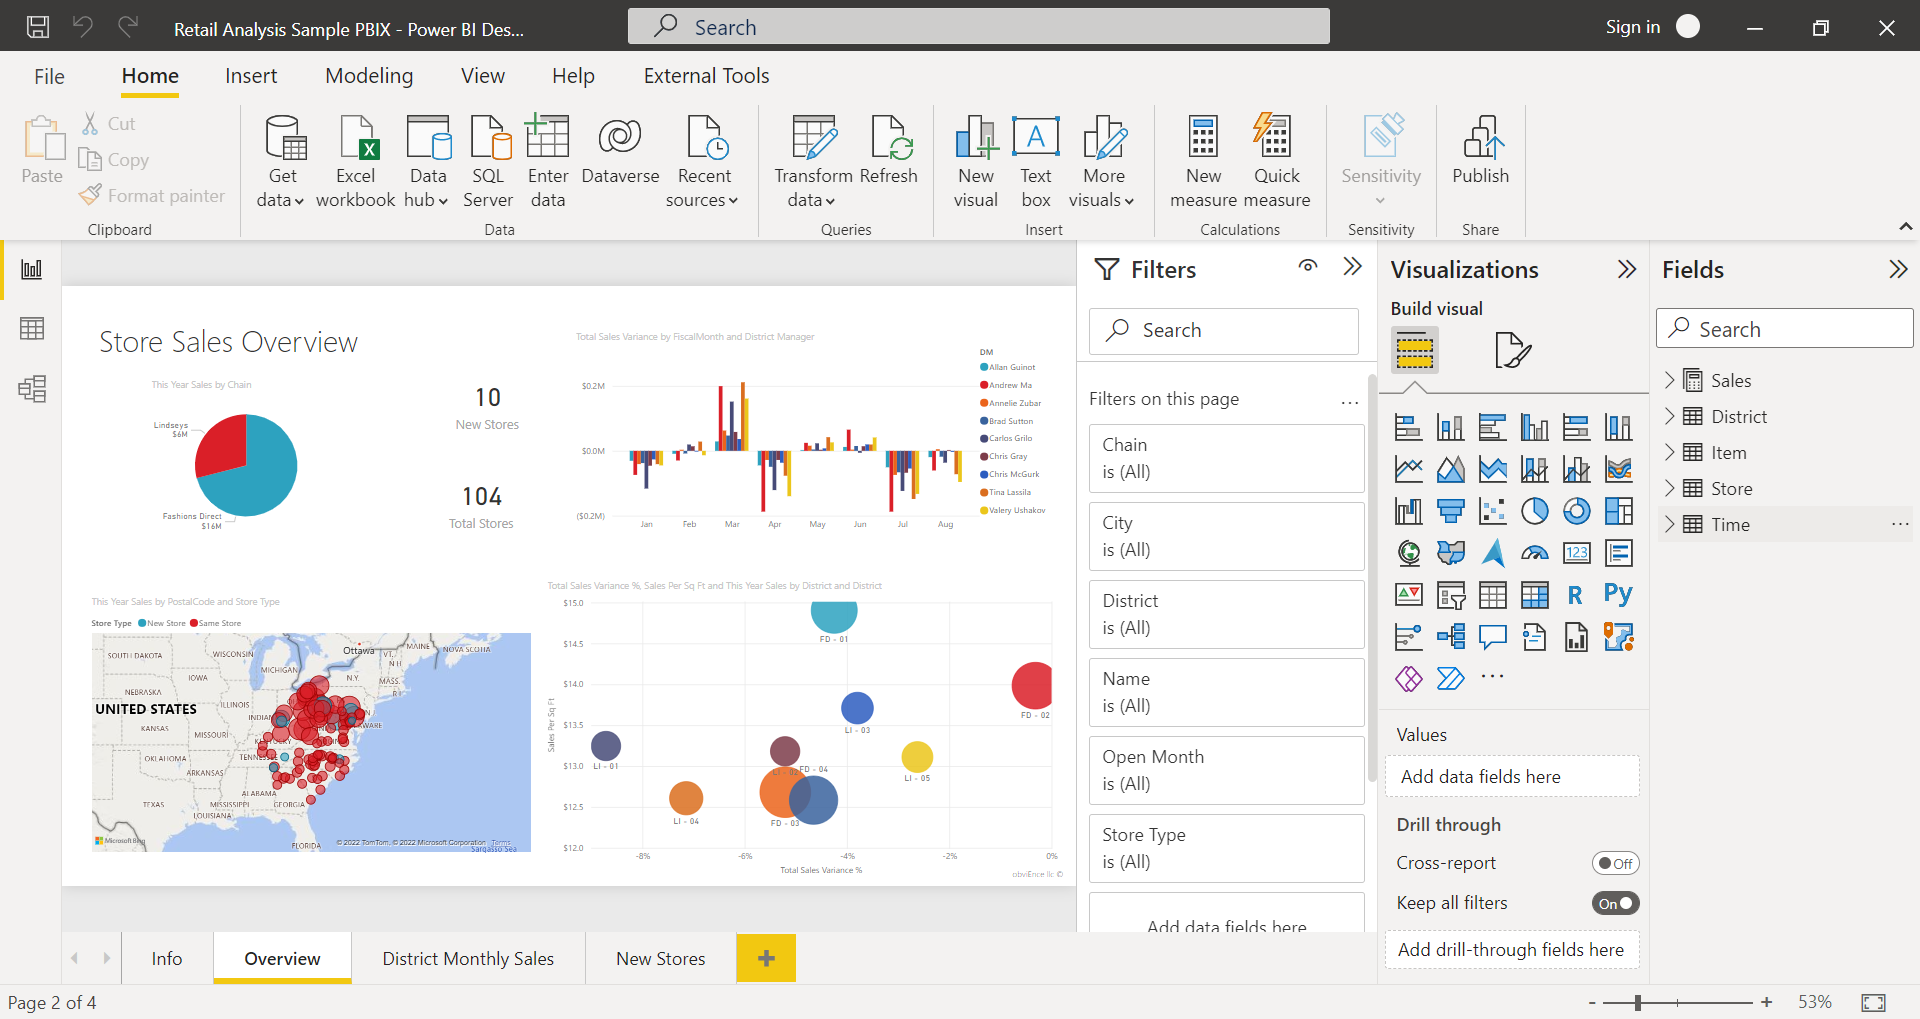
\includegraphics[width=0.75\linewidth]{img/PowerBIUI.png}
    \caption{Prostředí Power BI — vytváření nástěnky, zdroj: Microsoft, 2023, dostupné z: \url{https://learn.microsoft.com/en-us/power-bi/fundamentals/media/desktop-what-is-desktop/what-is-desktop-01.png} }
    \label{fig:PowerBIUI}
\end{figure}

\subsubsection{Určení}
Power BI je zejména vhodný pro střední až větší firmy, v nichž je potřeba rychle vytvářet vizualizace a nástěnky bez nutnosti rozsáhlého školení. Pro zkušenější uživatele nabízí řadu pokročilejších funkcí\cite{PowerBIBigCompanies:online}.

\subsubsection{Shrnutí}
Microsoft Power BI je velmi oblíbený nástroj pro business intelligence, který nabízí jak základní funkcionalitu většiny BI nástrojů, tak pokročilé analytické funkce, jako jsou Quick Insights, AI Insights a Analyze feature.

Co se týče našich požadavků na funkcionalitu, Power BI rozhodně oba dva splňuje, přičemž přenositelnost je zajištěna možností vytvářet a využívat zmíněné \hyperref[subsubsec:PowerBITemplates]{šablonové řešení}.

\subsection{Tableau}
-
% Tableau Desktop je výkonný nástroj pro vizualizaci dat, který umožňuje připojení, analýzu a vizualizaci jakýchkoli dat.

\subsubsection{Podporované zdroje dat}
-
% Připojení k datům: Tableau Desktop umožňuje připojení k datům jak na místě (on-premise), tak v cloudu.

\subsubsection{Výhody}
-
% Analýza dat: Uživatelé mohou provádět pokročilé analýzy, vytvářet vypočítaná pole, hledat shluky v datech, počítat procenta a používat různé nástroje k prozkoumání a kontrole dat2. Tableau Desktop také nabízí funkci výrazů úrovně detailu (LOD), které umožňují výpočty na úrovni zdroje dat a vizualizace.

% Vizualizace dat: S intuitivním rozhraním přetahováním a pomocí dynamických náhledů mohou uživatelé snadno vytvářet a iterovat vizualizace.

% Automatizované doplňkové informace: Tableau Desktop pomáhá lidem na všech úrovních dovedností lépe rozhodovat s daty. Nabízí zkušenosti zlepšené umělou inteligencí a strojovým učením, které vedou obchodní uživatele k odpovědím, které potřebují.

\subsubsection{Určení}
-
% Sdílení a spolupráce: Uživatelé mohou bezpečně sdílet analýzy a náhledy připojením k Tableau Serveru nebo Tableau Cloud.

\subsubsection{Shrnutí}
-
% Tableau Desktop je tedy komplexní nástroj, který nabízí širokou škálu funkcí pro práci s daty, od připojení k datům až po sdílení výsledků analýzy. Je to jakýsi laboratoř, ve které můžete objevovat význam, který se skrývá ve vašich datech

\subsection{Metabase}
- 
% Metabase je platforma pro analýzu dat, která umožňuje vyhledávání dat na vysoké úrovni po celém pracovním prostoru nebo detailnější dotazy, které lze vytvořit pomocí nízko-kódového SQL dotazovacího nástroje. 

\subsubsection{Podporované zdroje dat} 
- 
% Metabase podporuje mnoho různých databází a datových skladů, což umožňuje prozkoumávat a učit se z dat, bez ohledu na to, kde jsou uložena1. Mezi podporované zdroje dat patří: ...

\subsubsection{Výhody} 
- 
% Metabase je oblíbený pro své uživatelsky přívětivé rozhraní, snadnou navigaci a cenovou dostupnost jako nástroj s otevřeným zdrojovým kódem10. Další výhody zahrnují: 

% Snadné použití: Metabase je velmi snadno použitelný a ideální pro marketingové a obchodní profesionály všech úrovní. 

% Flexibilita: Metabase je známý svou flexibilitou pro více podniků v různých odvětvích nebo oblastech, stejně jako pro celkovou velikost organizace

% Podpora prostředí: Metabase je snadno nasaditelný a použitelný i pro netechnické uživatele díky podpoře prostředí. 

% Vizualizace dat: Metabase nabízí širokou škálu nástrojů pro vizualizaci dat, které umožňují vytváření komplexních zpráv a řídicích panelů. 

\subsubsection{Určení} 
- 
% Metabase je zaměřen na týmy pro analýzu dat v organizaci5. Je ideální pro malé a střední podniky, startupy nebo týmy s omezenými znalostmi BI. 

\subsubsection{Shrnutí}
- 
% Metabase je komplexní nástroj, který nabízí širokou škálu funkcí pro práci s daty, od připojení k datům až po sdílení výsledků analýzy. Jeho snadné použití, flexibilita a široká podpora datových zdrojů ho činí silným nástrojem pro jakoukoli organizaci, která se snaží získat cenné informace z jejích dat. 

% \subsubsection{TODO}
% SaaS deployment manažer
% Vzpomenout ten v Go,
% Mnoho nepotřebných features

\section{Závěr}\label{sec:AnalysEnd}

V předchozích sekcích jsme si představili několik nástrojů, jejichž kombinací lze splnit požadavky na funkcionalitu definované v~\hyperref[chap:analysis]{úvodním textu} této kapitoly. 
Ovšem kombinace těchto nástrojů by vytvářela poměrně nesourodý celek, který by bylo složité automatizovat a~integrovat do jednoho systému. 

Další problém představují nástroje na integraci dat.
Jsou totiž spíše určeny pro použití experty na integraci či analýzu dat, proto je u~nich kladen důraz na obecnost a~širokou škálu využití, a~tak pro náš systém mnohonásobně převyšují požadovanou funkcionalitu.
Tato nepotřebná funkcionalita přidává na komplexitě těchto nástrojů, což vytváří barieru pro použití ve spolupráci se zákazníkem - laikem.

V dalších kapitolách se tedy budeme soustředit na navržení a~implementaci vlastního řešení, které minimalizuje nabízenou funkcionalitu na nezbytně nutnou úroveň, jež splňuje funkční požadavky, za účelem zachování jednoduchosti použití.
Krom toho se budeme snažit vyhovět dalším požadavkům firmy na vlastní řešení.

Kdybychom přeci jen měli vybrat nejlepší hledanou kombinaci z představených nástrojů, byly by jí nástroje \textit{SSIS} a \textit{Power BI} od Microsoftu, které díky jednotnému původu nabízí nejsnadnější integrovatelnost.
